
%*****************************************
\chapter{Developing an Interaction System}\label{ch:forth}
%*****************************************
We developed an interaction system called \underline{\textbf{FiPa}} to further examine findings of Anonymous et al. \cite{anonymous}, discussed in Chapter \ref{ch:third}. Before entering into the development process, it is crucial to mention that the following interaction system was created solely to serve as a tool in the user case study, which we will present in Chapter \ref{ch:fifth}. The system is in no means a suggestion for an authentication concept and was not intended to be utilized as such. Its sole utilization and purpose was meant for the scope of this thesis, and no further. Therefore certain aspects ( e.g., security and effectiveness ) have consciously not been considered during the design and the development of this system. Nonetheless, during its creation, we tried our best to follow the steps of a \textbf{User-Centered Design} (UCD) approach and included a selection of \textbf{Human Computer Interaction} (HCI) principles, in order to make the system easier to understand and function. It was important to make sure that our design and structure choices, neither distracted our future study participants from the important factors of the study nor complicated the effort needed to concentrate on them.  


\section{Requirements of the Concept} \label{4.1}
As mentioned above, the interaction system was intended to be utilized as a tool to help examine certain factors later on in our study. These factors were \textbf{orientation time} and \textbf{input time}, previously presented in Chapter \ref{ch:third}. In order to do so, the interaction system had to be based on a certain concept. This concept had to be divided into two coherent and related small tasks: a \textbf{mental task} and a \textbf{practical task}. The intention behind this division was to be able to measure the \textbf{orientation time} \underline{(duration of the mental task)} and the \textbf{input time} \underline{(duration of the practical task)}, separately. Therefore, a built-in timer was required to undertake the measurements, which would be automatically saved in a database (Section \ref{4.3}).\\

In order to validate the findings of Anonymous et al. \cite{anonymous}, presented in Chapter \ref{ch:third}, we had to find a way through which we could examine the real effect that \textbf{orientation time} had on the perceived efficiency of an authentication concept, with respect to the \textbf{input time}. We, therefore, decided to analyze the following two contrasting time ratios:  
\begin{center}
    \textcolor{blue}{Long} orientation - \textcolor{red}{Short} input \\
    \textbf{vs.} \\
    \textcolor{red}{Short} orientation - \textcolor{blue}{Long} input.
\end{center} 

To have a baseline to which we could later compare the measured times of the ratios above, we included a third ratio, where orientation time and input time were equally long. We call this:  
\begin{center}
\textcolor{red}{Short} orientation - \textcolor{red}{Short} input.
\end{center} 

In contrast to the study by Anonymous et al. \cite{anonymous}, we wanted to directly examine the influence of \textbf{orientation time}, by comparing both contrasting ratios against each other, using \textit{only one concept}, instead of three (Chapter \ref{ch:third}). We hoped that by unifying all ratios into one concept, we could eliminate the possibility that our future participants' perceptions could be influenced by their personal preference of a particular concept. Therefore, the concept had to be malleable in a way, such that the time needed to accomplish the small tasks, could be modified by adjusting their degree of difficulty and complexity. We figured that the less difficult and the less complex a task was, the lesser time it needs to be accomplished, and vice versa. This assumption applied to both, \textbf{mental} and \textbf{practical task}.

\begin{figure}[t!]
\centering
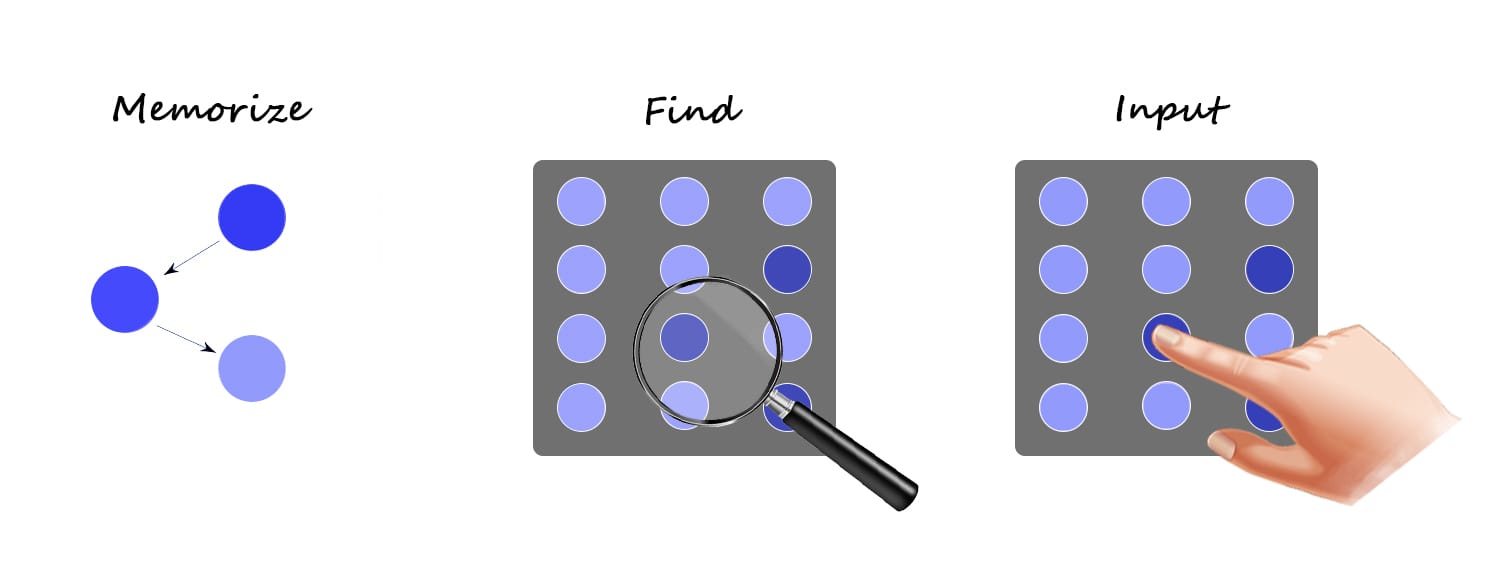
\includegraphics[width=15cm, height=6cm]{Chapters/graphics/ConceptIdea.jpeg}
\caption{Simple illustrtation of the idea. The procedure is composed of three steps: \textbf{Memorize} a pattern, \textbf{Find} the pattern, hidden inside a grid, and then \textbf{Input} of the pattern.}
\label{fig:concept}
\end{figure}

\section{Concept Development} \label{4.2}

In the following section, we will present the design and evaluation attempts that were necessary to generate \underline{\textbf{FiPa}}: the interaction system presented and utilized in our study. 

\subsection{Fundamental Concept Idea} \label{4.2.1}
We were interested in creating a concept that activated an interaction that believably resembled a smartphone authentication. We believed that by making the interaction similar to an authentication process, we could help our future participants better understand and adapt to the context of our study. That way, we hoped to receive more focused and detailed qualitative results. One of our goals was to construct a concept that was as usable as possible.  That way, we could shine the light on the actual usability issues which we intended to examine. We, therefore, decided to create a \textit{graphic-based concept}. Recent research has shown them to take longer to authenticate and to be more error-prone than alphanumeric approaches \cite{AnatomySmartphone}. However, they were still perceived as most user-accepted and were considered more comfortable to use, on average \cite{PatternWild}. To better understand the basic idea of our concept, we recommend referring to Figure \ref{fig:concept}, while reading our explanation: \\ 

The name of our concept, \underline{\textbf{FiPa}}, is inspired by its functionality. \underline{\textbf{FiPa}} is an abbreviation for the phrase "\underline{\textbf{Fi}}nd \underline{\textbf{Pa}}ttern" and its meaning will be comprehensible through the following description of its procedure: First, a predefined pattern is presented which has to be memorized well by the user. This pattern consists of a certain combination of buttons. Each button has a certain characteristic, that makes it distinguishable from others. Memorizing the order of the buttons and their distinct characteristics is premise for successfully accomplishing \textbf{mental} and \textbf{practical task} (Section \ref{4.2.1}). After \underline{memorizing} the pattern, a large grid, filled with buttons, is presented. The \textbf{mental task} thereby is to \underline{find} the memorized pattern, hidden in the grid. When found, the \textbf{practical task} is to \underline{input} the found pattern correctly into the grid (see figure \ref{fig:concept}).\\


We derived the idea of using a grid of buttons from the concept \textit{Pattern Rotation} \cite{Marbles, anonymous}. The choice of using specific characteristics for each button was inspired by the concept \textit{Marbles} \cite{Marbles, anonymous}. We tried to limit the amount of mental effort required for interacting with the concept by making a few intentional design choices. We imagined that having to reproduce the memorized pattern for the input completely, would be tiresome and not possible for every participant. We also took into consideration that the pattern would most certainly not be memorized permanently and would, therefore, be stored in their short-term memory. To that, we assumed that searching for the pattern would require less mental effort than its complete reproduction. That way, during the mental task, when the user stumbles upon the hidden pattern in the grid, they are more likely to detect it because they recognize it. So, by decreasing the amount of mental effort required for the interaction with the concept, we hoped that our participants would be able to shift their focus onto the different ratios in our study.

\begin{figure}[t!]
\centering
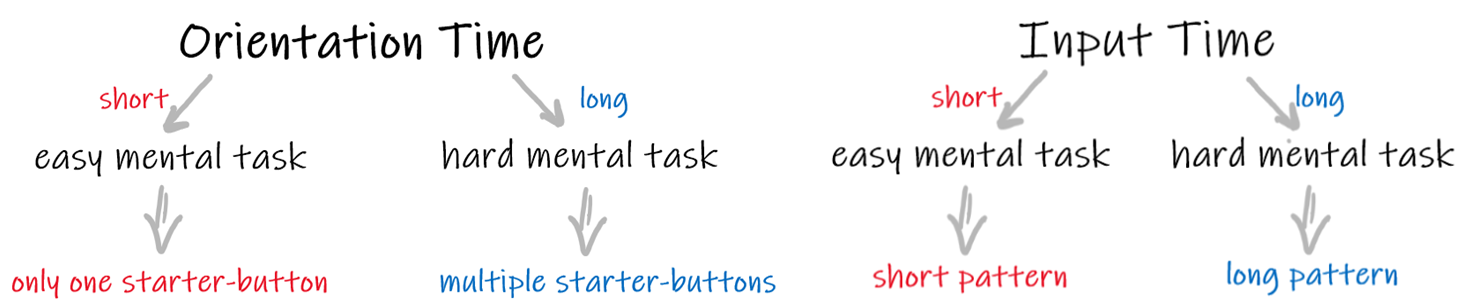
\includegraphics[width=13cm, height=4cm]{Chapters/graphics/OriInput.PNG}
\caption{Depiction of how we attempted to construct the mental and practical tasks, depending on whether \textbf{orientation time} and \textbf{input time} were long or short.}
\label{fig:orientation_input}
\end{figure}


\subsection{Concept Design} \label{4.2.2}
In the following we will present the design approaches that lead us to creating and developing the interaction system \underline{\textbf{FiPa}}.

\subsubsection{First Draft} \label{4.2.2.1}
We illustrated our initial vision for the design in figure \ref{fig:firstdraft}. As in \textit{Marbles} \cite{Marbles, anonymous}, we decided to make the different elements of our concept (the buttons) distinguishable through small images, emojis to be exact. We will first begin by explaining how we visualized the \textbf{practical task} and then proceed with explaining our intentions regarding the \textbf{mental task}. As mentioned in Section \ref{4.1}, a pattern is required to be memorized at the very beginning of the activity. To mark the beginning of a pattern, we determined the first button of each pattern to contain a key-emoji (see figure \ref{fig:firstdraft}). We will call this button the \textit{starter-button}. In order to modify whether the intended \textbf{input time} should be short or long, we created examples of how we imagined the patterns should look like in Figure (see figure \ref{fig:firstdraft}). Similar to the input method in \textit{Android Unlock Pattern}, we decided the user would enter the pattern by connecting the buttons with their finger. We found this input method to be more suitable, being that \underline{\textbf{FiPa}} was intended to be a smartphone application and that the user would interact with it through a touch screen. \\

As for the \textbf{mental task}, we envisioned to design a grid filled with emoji-buttons. The design of the grid depended on whether long \textbf{orientation time} or short \textbf{orientation time} was intended. As mentioned earlier in Section \ref{4.1}, we assumed that for a long \textbf{orientation time}, we need to create a difficult and complex search process. We imagined that by incorporating multiple \textit{starter-buttons}, besides the one belonging to the hidden pattern, we could complicate and elongate the search process in practice. In contrast, we imagined it would be possible to facilitate the pattern search, by having the only \textit{starter-button} in the grid belong to the hidden pattern. That way, our future participants could spot the pattern much easier and quicker. 

\begin{figure}[t!]
\centering
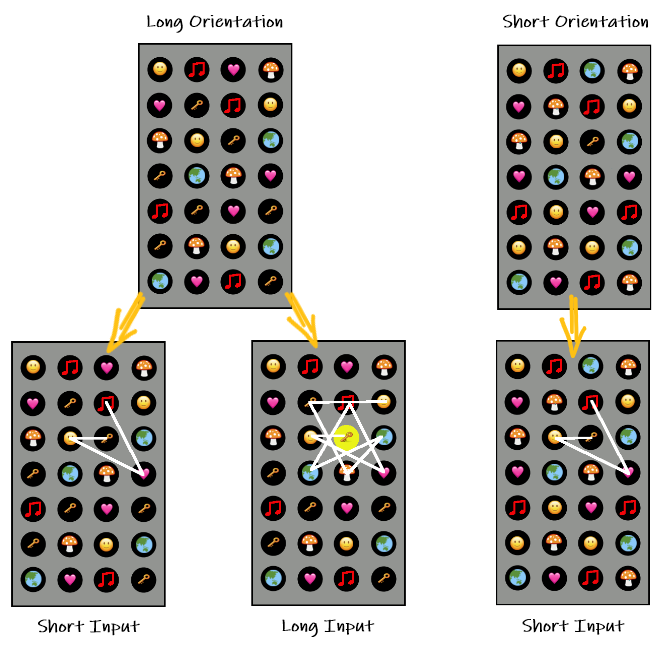
\includegraphics[width=14cm, height=14cm]{Chapters/graphics/firstdraft.PNG}
\caption{More detailed representation our vision for the design and the construction of the mental and practical tasks in our concept.    }
\label{fig:firstdraft}
\end{figure}

\subsubsection{Evaluation: First Draft} \label{4.2.2.2}
In order to find out if our concept was effective in practice, we created a paper prototype. The prototype encompassed the three ratios (Section \ref{4.1}) and was composed of three patterns\footnote{Two short patterns intended for \textit{short input time} and one long pattern intended for \textit{long input time}.} and three grids\footnote{Two grids with only one \textit{starter-button}, for \textit{short orientation time} and one grid with multiple \textit{starter-buttons}, for \textit{long orientation time}.}. We were able to gather six participants to evaluate our prototype. It was important for us to see how our design affected the usability of our concept. We wanted to ensure that it was easy to use and easy to understand.

Before the interaction, we roughly explained the purpose of our study and the functionality of our prototype. We used a form of \textit{Wizard Of Oz} prototyping \cite{Butz2014}. During the interaction, we would uncover the following event of the prototype (grid or pattern), depending on the participant's \textit{input} or \textit{action}. We timed the interaction for each user in a specific manner, using a stopwatch. Our intention was to ensure that the accomplishment of the \textbf{mental task}, designed for long \textbf{orientation time}, truly took longer than the ones intended for short \textbf{orientation time}. The same was important for the \textbf{practical tasks} and their corresponding \textbf{input times}. We wanted to measure the ratios similar to the approach made by Anonymous et al. \cite{anonymous} (Chapter \ref{ch:third}). Therefore, we determined a starting and ending point for each of the tasks. Thereby we set a clear time interval for each of the phases: \textit{orientation} and \textit{input}. A \textbf{mental task} began right after a particular grid was uncovered and ended as soon as the hidden pattern was found. The find was indicated by tapping the \textit{starter-button} of the pattern once. The \textbf{practical task} began with the \textit{first button press} and ended with the very \textit{last button press}.  For the input, the \textit{starter-button} had to be tapped once again, even though it had previously been tapped to signify the find. We were aware that the measured times would not be completely accurate. They were only intended to serve as a rough estimate of the phases.\\


Five of the participants considered the emojis to be overwhelming on the eyes. They found that it made the grid appear very crowded. Moreover, the long pattern was considered too complicated and was hard to memorize by all of the participants (see figure \ref{fig:firstdraft}). Regarding the input method, we noticed that it was not suitable for realizing the different variations of \textbf{input time} that we wanted to achieve. Although it worked well for short \textbf{input time}, the time needed to enter the long pattern was not as long as we had intended for it to be.
Luckily, the idea behind the concept was liked by all of the participants. Especially, the notion of starting each pattern with a specific \textit{starter-button}. Despite the flaws mentioned above, they understood the basic functioning of our concept well. \\

The information gained and the lessons learned through the previous evaluation phase gave us a closer insight into humans' perception and cognitive ability. At this point, we were one step closer to creating a more usable and effective interaction system.

\begin{figure}[t!]
\centering
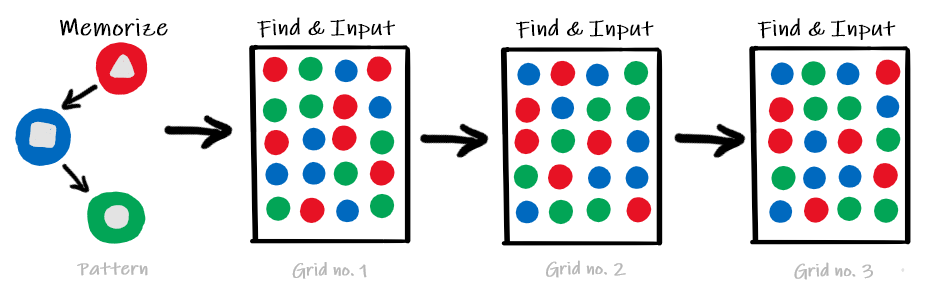
\includegraphics[width=13cm, height=5cm]{Chapters/graphics/seconddraft.PNG}
\caption{A sketch that presents the basic structure of each phase of the prototype. Each grid represents a \textbf{couple}: a mental and a practical task. After memorizing the given pattern, three uniquely designed grids followed. The pattern had to be found and entered in each of the grids, one after the other.}
\label{fig:secondDraft}
\end{figure}

\subsubsection{Second Draft} \label{4.2.2.3}

We decided to make a few adjustments regarding the overall aesthetics and the design of our concept. Through further research, we learned that due to the \textit{pictorial superiority effect} \cite{pictorial}, humans can retain information through images, much better than through letters or numbers \cite{pictorial, 2014}. That is why we chose to continue representing the characteristics of the buttons through images. We decided to reduce the crowded appeal of the previous draft by replacing the emojis with three simple shapes: \textit{circle}, \textit{square}, and \textit{triangle}. Our initial choice of colors for the design was: \textit{red}, \textit{green} and \textit{blue}. The reason for our choice is that they are the basic colors that the human eye perceives naturally \cite{Butz2014}. We kept the notion of each pattern, beginning with a \textit{starter-button} and decided for it to be red containing a triangle, as illustrated in [FIGURE]. We chose the triangle because it is a symbol that has been shown to convey the meaning of \textit{power}\footnote{http://www.whiteriverdesign.com/meaning-shapes-design/ - last accessed: 2019/11/16} and \textit{permanence} \cite{Frutiger1998}.  Moreover, the human eye is naturally attracted to its shape \footnote{https://designshack.net/articles/layouts/the-sometimes-hidden-meaning-of-shapes/ - last accessed: 2019/11/16}. We assumed that through the mentioned effect of the triangle and the alerting appeal of the color red, we could attract the user's \textit{pre-attentive perception} \cite{Butz2014} to these buttons. \\

Next, we proceeded with the pattern and grid design. After a couple of trials, we determined the size of the grid to be 4x7, because we found that the size was big enough to hold a decent amount of buttons and yet suitable enough to not overly confuse our future participants during the interaction. Also, we decided to incorporate so-called \textit{traps} into the grids. \textit{Traps} are a set of buttons, that have a similar constellation and set of characteristics as the hidden pattern, yet are not identical to it. Their purpose was to mislead the user, during the \textbf{mental task} and thereby elongate the searching process. Another modification made was the input method. We found that by tapping all of the buttons in the right order, rather than connecting them (Section \ref{4.2.2.1}) we could gain more control of the approximate duration for the input even better. While creating the patterns, they needed not to take up too much space in the grid. That way, we could shuffle the buttons and set \textit{traps} much more freely. 

\begin{figure}[t!]
\centering
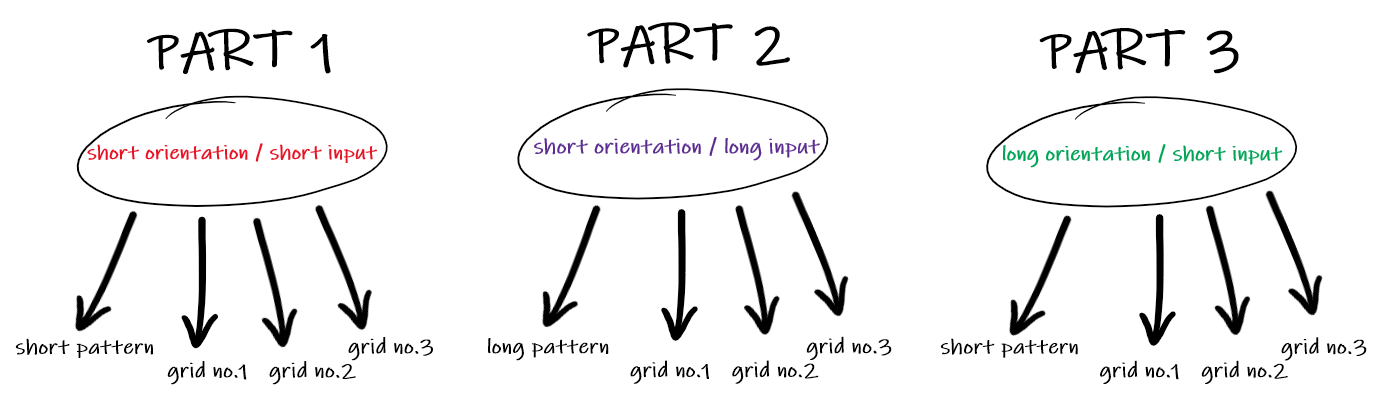
\includegraphics[width=13cm, height=5cm]{Chapters/graphics/prototypeStructure.PNG}
\caption{Simple representation of the structure of our second prototype. Each part is assigned to a particular ratio. For each ratio there are three grids. Each grid presents a \textbf{mental task} (find) and \textbf{practical task} (input), a so called \textbf{couple}. The order of the ratios presented in this figure is only a suggestion. The exact order of the ratios was not important in the evaluation phase.}
\label{fig:prototype}
\end{figure}

\subsubsection{Evaluation: Second Draft} \label{4.2.2.4}

As in our first draft evaluation (Section \ref{4.2.2.2}), we created a \textit{Wizard of Oz} paper prototype \cite{Butz2014} to evaluate the changes and improvements that we made in our concept. However, this time, the prototype was created differently. We wanted to test a certain structure to see if it would be suitable for the implementation of our concept. The prototype was structured into three parts thus, we have three ratios (Section \ref{4.1}) to examine. In the previous draft, we only had one \textbf{mental} and \textbf{practical task} per ratio. For simplicity, we will call the composition of \textbf{mental} and \textbf{practical task}, a \textbf{couple}. Instead of having only one couple per ratio, we decided it would be reasonable to assign three to each ratio. That way, our participants would have the chance to interact with each ratio-designs more than once and remember them better during the qualitative segment of our study. Figure \ref{fig:prototype} represents the rough structure of our paper prototype. We tested our prototype with the same set of participants with whom we had tested our first draft. We did so, in order to receive a more detailed feedback on whether the flaws, detected in our first draft, were correctly fixed. It was possible to interview the same set of participants because the design and the structure of the \textbf{mental} and \textbf{practical tasks} were completely different than in the first draft. Fortunately, both, layout and structure of our prototype were accepted well. \\

We adapted the same measurement method that we used in Section \ref{4.2.2.2}. We considered the first and second couple of each part to be an exercise for the participant to get acquainted with the concept. Therefore, we only considered the average times of each third couple of each ratio. Although not accurate, the approximate duration resulted as we had imagined and desired for our concept.

\section{Implementation of the Concept} \label{4.3}



